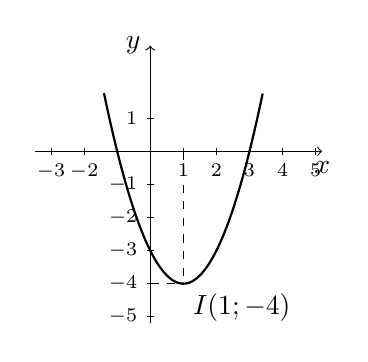
\begin{tikzpicture}[scale=0.42]
    \draw[->] (-3.5,0) -- (5.2,0) node[below] {$x$};
    \draw[->] (0,-5.2) -- (0,3.2) node[left] {$y$};

    \foreach \x in {-3,-2,1,2,3,4,5}
        \draw (\x,0.1) -- (\x,-0.1) node[below] {\scriptsize $\x$};

    \foreach \y in {-5,-4,-3,-2,-1,1}
        \draw (0.1,\y) -- (-0.1,\y) node[left] {\scriptsize $\y$};

    \draw[smooth, samples=200, domain=-1.4:3.4, thick]
        plot (\x, {\x*\x - 2*\x - 3});

    \draw[dashed] (1,0) -- (1,-4);
    \draw[dashed] (0,-4) -- (1,-4);
    \fill (-1,0) circle (1.3pt);
    \fill (3,0) circle (1.3pt);
    \fill (1,-4) circle (1.3pt);
    \node[below right] at (1,-4) {$I(1;-4)$};
\end{tikzpicture}
